\documentclass{report}


%%%%%%%%%%%%%%%%%%
%   Liste des packages utilisés  %
%%%%%%%%%%%%%%%%%%

% (oui y'en a 95% qui sont inutiles ^^)

\usepackage{amssymb}
\usepackage{array}
\usepackage{hyperref}
\usepackage{booktabs}
\usepackage{multirow}
\usepackage{float}
\usepackage{lmodern} %Pack de police
\usepackage{color}
\usepackage[dvipsnames]{xcolor}
\usepackage{graphicx}
\usepackage[utf8x]{inputenc}
\usepackage[T1]{fontenc}
\usepackage{natbib}
\usepackage[francais]{babel}
\usepackage{caption}
\usepackage{listings}
\usepackage{booktabs}
\usepackage[top=2cm, bottom=2cm,left=2cm, right=2cm]{geometry}
\usepackage{blindtext}
\usepackage{setspace}
\usepackage{graphicx}
\usepackage{titlesec, blindtext, color} % titres spéciaux + couleur pour les chapter

% on transforme les chapters en juste le numéro suivi du titre, avec un barre grisse
\definecolor{gray75}{gray}{0.75}
\newcommand{\hsp}{\hspace{20pt}}
\titleformat{\chapter}[hang]{\Huge\bfseries}{\thechapter\hsp\textcolor{gray75}{|}\hsp}{0pt}{\Huge\bfseries}

\begin{document}


%%%%%%%%%%%
%  Page de garde  %
%%%%%%%%%%%
\begin{titlepage}
	\begin{center}
	
		\begin{spacing}{1.5}
			Projet Picross\\
			\vspace*{\fill}
		\end{spacing}
		
		\begin{spacing}{2.5}
			\textbf{\Huge Application de création et d'aide à la résolution de puzzle \textit{picross}}\\[0.5cm]
			\textbf{\huge Cahier d'analyse et conception} \\
			\vspace*{\fill}
			\textit{Étudiants :}
		\end{spacing}

		\begin{spacing}{1.15}
			\large
			\textsc{Brinon} Baptiste\\
			\textsc{Brocherieux} Thibault\\
			\textsc{Cohen} Mehdi\\
			\textsc{Debonne} Valentin\\
			\textsc{Lardy} Anthony\\
			\textsc{Mottier} Emeric\\
			\textsc{Pastouret} Gilles\\
			\textsc{Pelloin} Valentin\\
			\vspace*{\fill}
			\textbf{Groupe n°2} \\
			\textnormal{\large Licence Informatique\\ Le Mans Université\\ \today}
		\end{spacing}
		
	\end{center}
\end{titlepage}


%%%%%%%%%%
%    Sommaire    %
%%%%%%%%%%
\renewcommand{\contentsname}{Sommaire}
\tableofcontents


\chapter{Présentation}

	\section{Introduction}

		Dans le cadre de l'unité d'enseignement "Génie logiciel 2" de la Licence d'informatique de Le Mans Université, les étudiants de troisième année sont amenés à travailler sur un projet de développement d'une application. \\
		Ce document décrit ...

	
 	\section{Objectif de l'application}		
		Nous devons réaliser un jeu de type picross (aussi appelé nonogramme, logigramme ou hanjie) permettant à un utilisateur de résoudre des grilles et de l'aider dans sa réalisation.
		
		\section{Outils}
		
		// Language logiciel ...
		
\chapter{Conception générale}

    \section{conduite de projet}
    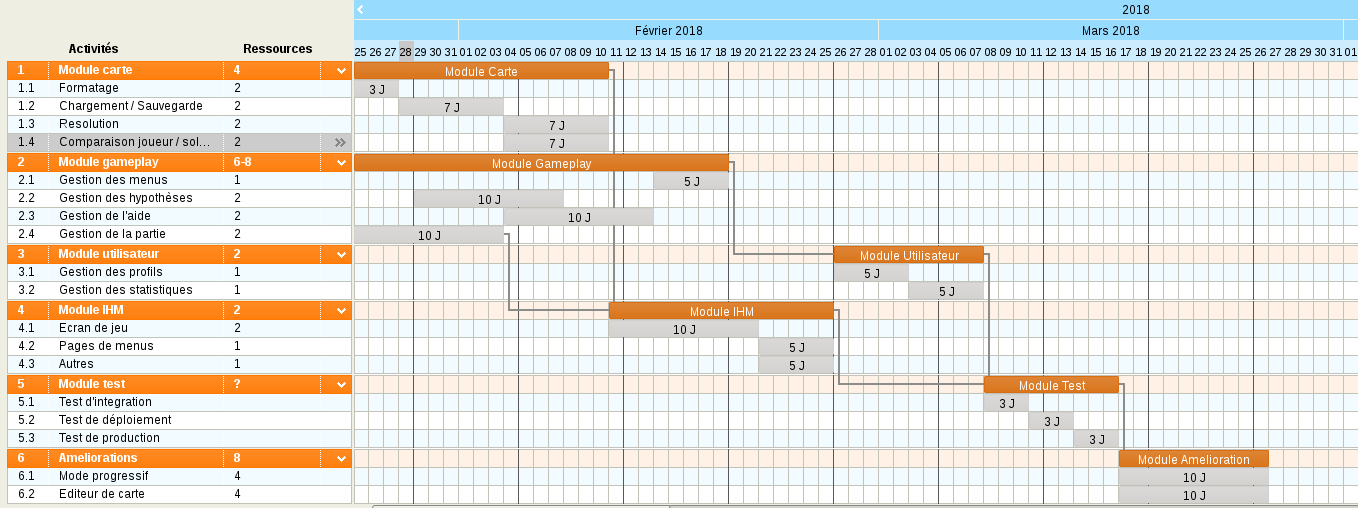
\includegraphics{../ganttDetaille.png}
    \\
     À travers ce diagramme de Gantt, nous observons l'organisation du projet sur les trois mois à venir. Le projet se découpe en plusieurs modules : carte, gameplay, utilisateur, IHM, test et améliorations.
    Chaque module a une durée de vie, nous lui accordons un temps de travail et un certain nombre de personnes, les modules sont également divisés en différentes étapes ce qui correspond aux fonctionnalités de l'application. Les modules sont imbriqués les uns dans les autres, c'est-à-dire que certains dépendent d'autres modules. Sans les modules gameplay et carte réalisés, le module IHM ne peut être réalisé. 
    
    \section{Fonctionnalité}
      // Cas d'utilisation + descriptif
      // diagrammes de séquences + descriptif 
    
		\section{Image}
			// Schéma liens entre écrans
			// Description
			
\chapter{Conception détaillé}

    \section{ ,, }
      // diagramme de classe + descriptif

    
\chapter{Annexes}

      // maquettes

\end{document}
